\chapter{Personalplaner}\label{personal:mitglieder}
Im Kopf des Fensters aus \cref{fig:personal:mitglieder} kann eingestellt werden welche Personen angezeigt werden sollen.
Ebenso kann durch einen Knopfdruck eine E-Mail an alle angezeigten Personen erstellt werden.
Werden bei dieser Aktion Personen gefunden, für die keine Mailadresse angegeben ist,
so können die hinterlegten Postadressen in einer CSV-Datei gespeichert werden.
Diese Daten können dann z.B.\ für Serienbriefe genutzt werden.


\begin{figure}[!h]
	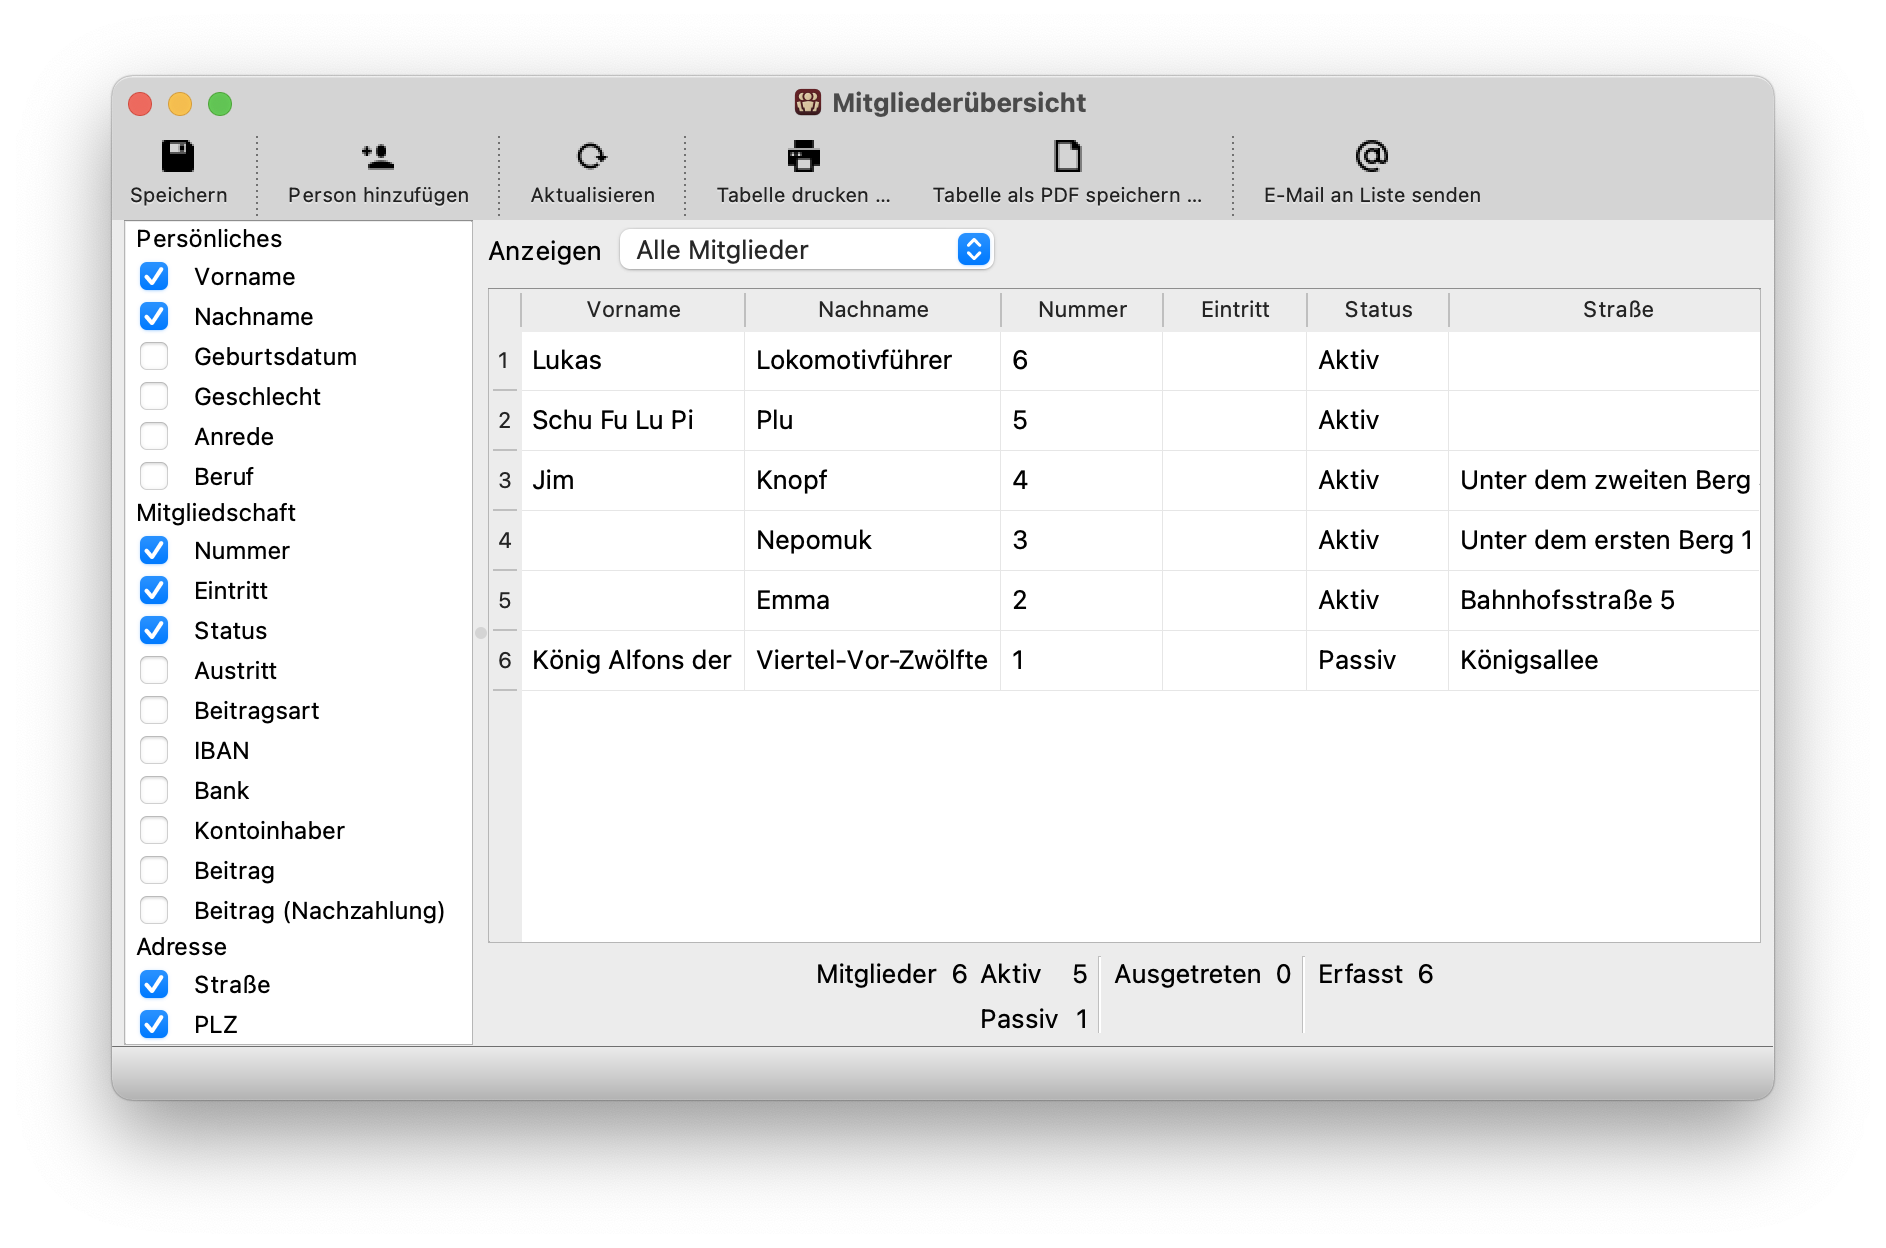
\includegraphics[width=\textwidth]{img/personal-liste}
	\caption{Die Mitgliederliste mit allen ausgewählten Mitgliedern.}
	\label{fig:personal:mitglieder}
\end{figure}

\begin{neu}
Die Einzelansicht einer Person kann über einen Doppelklick auf eine Zelle der entsprechenden Zeile geöffnet werden.

Über eine ent- bzw.\ zusammenfaltbare Liste auf der linken Seite des Fensters kann eingestellt werden,
welche Daten in der Tabelle angezeigt werden.
\end{neu}
Im unteren Bereich des Fensters wird eine kurze Statistik
der aktuellen und ausgetretenen Mitglieder angezeigt.

\paragraph{Export}
Die Tabelle kann über die Knöpfe \button{Tabelle drucken} und \button{Tabelle als PDF speichern} ausgegeben werden.
Über das Menü \aktion{Exportieren} steht noch ein Export als CSV-Datei zur Verfügung (hier werden alle gespeicherten Daten exportiert),
sodass die Daten in anderen Programmen verarbeitet werden können.
Ebenso besteht die Möglichkeit über den Eintrag \aktion{Stammdatenblätter} die Daten eines Mitglieds bzw.\ aller angezeigten Personen auszugeben.
Hierbei wird für jede Person eine Seite erzeugt, die in einem gemeinsamen Dokument gespeichert werden.
